%%%%%%%%%%%%%%%%%%%%%%%%%%%%%%%%%%%%%%%%%%%%%%%%%%%%%%%%%%%%%%%%%%%%
% Author: A. Herrera Poyatos
% Tittle: Continuidad y diferenciabilidad de la solución 
% respecto de condiciones iniciales y  parámetros
%%%%%%%%%%%%%%%%%%%%%%%%%%%%%%%%%%%%%%%%%%%%%%%%%%%%%%%%%%%%%%%%%%%%%


\newpage

\section{Estabilidad en el sentido de Lyapunov}

Estudiamos el principal concepto de estabilidad en teoría de ecuaciones diferenciales, aunque
existen otros conceptos.


\begin{definition}
  Sea $D \subset \R \times \R^d$ abierto y $f \colon D \to \R^d$ localmente lipschitziana respecto
  de la segunda variable. Sea $\varphi\colon ]\alpha, +\infty[ \to \R^d$ una solución maximal de
  $x' = f(t,x)$. Diremos que $\varphi$ es una solución estable de \eqref{eq:edo} en el sentido de
  Liapunov si para todo $\varepsilon >0$ existe $\delta > 0$ tal que si $(t_0, x_0) \in D$ y
  $||x_0-\varphi(t_0)|| \le \delta$, entonces $\omega(t_0, x_0) = +\infty$ y
  $||X(t, t_0, x_0) - \varphi(t)|| < \varepsilon$ para todo $t \ge t_0$.
\end{definition}

\begin{remark}
  Aunque parece que $t_0$ juega un papel esencial en la definición en la realidad no lo hace por el
  Teorema de dependencia continua respecto de condiciones iniciales.
\end{remark}

\begin{ex}
  Veamos ejemplos de soluciones estables y no estables.
  \begin{enumerate}
  \item $x' = 0$.
  \item Consideramos la EDO $x' = -x$. Es estable...
  \item Consideramos la EDO $x' = -x^2$. Es estable...
  \item Consideramos la EDO $x' = x$. Su solución general es $X(t,0,x_0) = e^t x_0$. Tenemos que
    $\omega(t_0, x_0) = +\infty$ pero no es estable.
  \end{enumerate}
\end{ex}

\begin{definition}
  Sea $D \subset \R \times \R^d$ abierto y $f \colon D \to \R^d$ localmente lipschitziana respecto
  de la segunda variable. Sea $\varphi\colon ]\alpha, +\infty[ \to \R^d$ una solución maximal de
  $x' = f(t,x)$. Diremos que $\varphi$ es una solución asintóticamente estable (AE) de
  \eqref{eq:edo} si existe $\mu > 0$ tal que si $(t_0, x_0) \in D$ verifica
  $||x_0 - \varphi(t_0)|| < \mu$, entonces $\omega(t_0, x_0) = +\infty$ y
  $\lim_{t \to +\infty} ||X(t, t_0, x_0) - \varphi(t)|| = 0$.
\end{definition}

\subsection{Estabilidad de EDOs lineales}

En esta sección estudiamos la estabilidad de EDOs lineales, en las que estas propiedades tendrán su
contraparte en términos de matrices fundamentales. Recordemos en este punto el concepto de EDO
lineal. Sean $I \subset \R$ abierto, $A \colon I \to \mathcal{M}_{d}(\R)$ y $b \colon I \to \R^d$
continuas.  Una \emph{EDO lineal} es una ecuación diferencial ordinaria de la forma
\begin{equation}
  \label{eq:lineal}
  x' = A(t)x + b(t).
  \tag{EL}
\end{equation}

Toda EDO lineal tiene asociada su \emph{ecuación homogénea }
\begin{equation}
  \label{eq:lineal:hom}
  x' = A(t)x.
  \tag{ELH}
\end{equation}

\begin{proposition}
  Sean $I = ]\alpha, +\infty[ \subset \R$, $A \colon I \to \mathcal{M}_{d}(\R)$ y
  $b \colon I \to \R^d$ continuas. Son equivalentes las siguientes afirmaciones:
  \begin{enumerate}
  \item Todas las soluciones de \eqref{eq:lineal} son estables.
  \item Existe una solución estable de \eqref{eq:lineal}.
  \item Todas las soluciones de \eqref{eq:lineal:hom} son acotadas en el futuro.
  \item Existe una matriz fundamental de \eqref{eq:lineal:hom} acotada en el futuro.
  \end{enumerate}
\end{proposition}
\begin{proof}
  Veamos que b) implica c). Supongamos que $\varphi\colon ]\alpha, +\infty[ \to \R$ es una solución
  estable de \eqref{eq:lineal}. Sea $\Psi \colon ]\alpha, +\infty[$ $\to \R$ solución de
  \eqref{eq:lineal:hom}. Dado $\varepsilon > 0$, existe $\delta > 0$ tal que para todo
  $(t_0, x_0) \in D$ con $\alpha < t_0$ y $||x_0 - \varphi(t_0)|| < \delta$ se tiene
  $\omega(t_0, x_0) = +\infty$ y $||X(t, t_0, x_0) - \varphi(t)|| < \varepsilon$. Sea
  $t_0 > \alpha$. Existe $\lambda > 0$ tal que $||\lambda \Psi(t_0)|| < \delta$. Por tanto, la
  solución $\varphi_1 = \varphi + \lambda \Psi$ está definida en $]t_0,+\infty[$ y verifica
  $||\Psi(t)||\le ||\varphi_1(t) - \varphi(t)|| < \varepsilon$ para todo $t > t_0$.

  Veamos que d) implica a). Sea $\Psi \colon ]\alpha, +\infty[ \to \R$ una matriz fundamental de
  \eqref{eq:lineal:hom} acotada en el futuro. Sea $\varphi \colon ]\alpha, +\infty[$ una solución de
  \eqref{eq:lineal}. Tenemos que
  \[ X(t, x_0) = \varphi(t) + \Psi(t) \Psi(t_0)^{-1} (x_0 - \varphi(t_0)). \] Sea $M > 0$ cota de
  $\Psi$. Para cada $\varepsilon > 0$ tomamos $0 < \delta < \varepsilon / (M
  ||\Psi(t_0)^{-1}||)$. Nótese que $\omega(t_0, x_0) = +\infty$ por el teorema de crecimiento a lo
  sumo lineal. Además, tenemos que $||X(t,x_0) - \varphi(t)|| z \varepsilon$ para todo $t \ge t_0$.
\end{proof}

Análogamente podemos demostrar el siguiente resultado referente a la estabilidad asintótica.
\begin{proposition}
  Sean $I = ]\alpha, +\infty[ \subset \R$, $A \colon I \to \mathcal{M}_{d}(\R)$ y
  $b \colon I \to \R^d$ continuas. Son equivalentes las siguientes afirmaciones:
  \begin{enumerate}
  \item Todas las soluciones de \eqref{eq:lineal} son asintóticamente estables.
  \item Existe una solución asintóticamente estable de \eqref{eq:lineal}.
  \item Todas las soluciones de \eqref{eq:lineal:hom} tienden a $0$ cuando $t \to +\infty$.
  \item Existe una matriz fundamental de \eqref{eq:lineal:hom} que tiende a $0$ cuando
    $t \to +\infty$.
  \end{enumerate}
\end{proposition}

Como consecuencia de estos resultados, el estudio de la estabilidad en ecuaciones lineales se reduce
en estudiar una matriz fundamental en $[t_0, +\infty[$.

\begin{ex}
  Sean $a, b \in \mathcal{C}(]\alpha, +\infty[, \R)$. Consideramos una EDO lineal de una variable
  \begin{equation}
    \label{eq:lineal:1}
    x' = a(t)x+b(t).
  \end{equation}
  Sea $A$ una primitiva de $a$. Una matriz fundamental de la ecuación homogénea es
  $\Psi(t) = \exp(A(t))$. Nótese que la matriz fundamental está acotada si, y solo si, $A$ está
  acotada superiormente, en cuyo caso existe $\{t_n\}$ tal que $\{a(t_n)\} \to 0$. Es más,
  $\lim_{t \to +\infty} \Psi(t) = 0$ si, y solo si, $\lim_{t \to +\infty} A(t) = -\infty$.
\end{ex}

Nos ocupamos a continuación del caso más simple, las ecuaciones lineales con coeficientes
constantes.  Sea $A \in \mathcal{M}_d(\R)$. Consideramos la ecuación
\begin{equation}
  \label{eq:lineal:cons}
  x' = A x, \quad t_0 = 0.
  \tag{LHC}
\end{equation}
La matriz fundamental principal en $t = 0$ es $\Phi(t) = \exp(At)$. Para su cálculo tenemos que
recurrir a la forma canónica de Jordan. Sea $\sigma(A) = \{\lambda_1, \ldots, \lambda_k\}$ el
conjunto de los valores propios de $A$. Denotamos por $\mathrm{m}(\lambda_j)$ a la multiplicidad
geométrica del valor propio $\lambda_j \in \sigma(A)$ y denotamos por $\nu(\lambda_j)$ al número
número de $1$ de la caja de Jordan asociada a $\lambda_j$. El teorema de Jordan dice que existen
$P, J \in \mathcal{M}_d(\mathbb{C})$ con $P$ invertible y $J$ diagonal por bloques, esto es,
\begin{equation}
  \label{eq:jordan}
  J = \left(
    \begin{matrix}
      J_1 & \cdots & 0 \\
      \vdots  & \ddots  & \vdots \\
      0 & \cdots & J_r
    \end{matrix}
  \right),
\end{equation}
donde $J_i \in \mathcal{M}_{\nu(\lambda_i)+1}(\mathbb{C})$ es de la forma
\begin{equation}
  \label{eq:jordan:bloque}
  J_i = \left(
    \begin{matrix}
      \lambda_i & 1 & 0 & \cdots & 0 \\
      0 & \lambda_i & 1 & \cdots & 0 \\
      \vdots  & \ddots & \ddots  & \ddots & \vdots \\
      0 &  \cdots & 0 & \lambda_i & 1 \\
      0 & \cdots & 0 & 0 & \lambda_i
    \end{matrix}
  \right),
\end{equation}
tales que $A = P J P^{-1}$. Este resultado nos permite calcular la exponencial de $A$ con facilidad
pues $\exp(At) = P \exp(Jt) P^{-1}$ y sabemos calcular la exponencial de $J$. En efecto,
$J_i = \lambda_i I + N$, donde $N$ tiene unos en la primera diagonal a la derecha de la diagonal
principal. Tenemos que $I \cdot N = N \cdot I$, luego $\exp(J_i t) = \exp(t \lambda_i I ) \exp(t N)$
y, fijado $k = \nu(\lambda_i)$, se cumple

\begin{equation}
  \label{eq:jordan:bloque}
  \exp(J_i t) = e^{t \mathrm{Re}(\lambda_i)} \left(
    \begin{matrix}
      1 & t & t^2 / 2 & \cdots & \frac{t^k}{k!} \\
      0 & 1 & t & \cdots & \frac{t^{k-1}}{(k-1)!} \\
      \vdots  & \ddots & \ddots  & \ddots & \vdots \\
      0 & \cdots & 0 & 1 & t \\
      0 & \cdots & 0 & 0 & 1
    \end{matrix}
  \right).
\end{equation}

En lo que sigue usaremos la notación
$\sigma_0(A) = \{\lambda \in \sigma(A) \mid \mathrm{Re}(\lambda) = 0\}$.

\begin{theorem}\label{thm:estabilidad:lineal:cte}
  Sean $A \in \mathcal{M}_d(\R)$ y $\mu = \max \{\mathrm{Re}(\lambda) \mid \lambda \in \sigma(A)\}$.
  \begin{enumerate}
  \item Si $\mu < 0$, entonces las soluciones de \eqref{eq:lineal:cons} son asintóticamente
    estables.
  \item Si $\mu = 0$ y $\nu(\lambda) = 0$ para todo $\lambda \in \sigma_0(A)$, entonces las
    soluciones de \eqref{eq:lineal:cons} son estables pero no asintóticamente estables.
  \item Si $\mu = 0$ y existe $\lambda \in \sigma_0(A)$ tal que $\nu(\lambda) \ge 1$, entonces
    \eqref{eq:lineal:cons} es inestable.
  \item Si $\mu > 0$, entonces \eqref{eq:lineal:cons} es inestable.
  \end{enumerate}
\end{theorem}
\begin{proof}
  Sean $J, P \in \mathcal{M}_d(\R)$ con $P$ invertible y $J$ matriz de Jordan tales que
  $A = P J P^{-1}$. Nótese que la acotación en el futuro y la existencia de límite en $+\infty$ de
  $\exp(A t)$ equivalen a la acotación en el futuro y la existencia de límite en $+\infty$ de
  $\exp(J t)$. La disyuntiva expuesta en el teorema es una consecuencia directa de
  \eqref{eq:jordan:bloque}.
\end{proof}


El Teorema \ref{thm:estabilidad:lineal:cte} es particularmente fácil de aplicar en el caso $d =
2$. En tal caso, la discusión se simplifica enormemente como muestra la Tabla
\ref{table:estabilidad}. Como consecuencia obtenemos el siguiente corolario.

\begin{table}[H]
  \centering
  \begin{tabular}{|cc|cc|l|}
    \hline
    \multicolumn{5}{|c|}{Valores propios reales} \\
    \hline
    $\lambda_1$ & $\lambda_2$ & Traza & Determinante & Clasificación \\
    \hline
    - & - & - & + & A.E. \\
    + & + & + & + & Inestable \\
    - & + & ? & - & Inestable \\
    - & 0 & - & 0 & Estable, no A.E. \\
    0 & + & + & 0 & Inestable \\
    0 & 0 & 0 & 0 & Inestable \\
    \hline
    \multicolumn{5}{|c|}{Valores propios complejos} \\
    \hline
    \multicolumn{2}{|c}{$\mathrm{Re}(\lambda_1)$} & Traza & Determinante & Clasificación \\
    \hline
    \multicolumn{2}{|c}{-} & - & + & A.E. \\
    \multicolumn{2}{|c}{+} & + & + & Inestable \\
    \multicolumn{2}{|c}{0} & 0 & + & Estable, no A.E.\\
    \hline
  \end{tabular}
  \caption{Estudio de la estabilidad el sistema \eqref{eq:lineal:cons} en términos de los valores
    propios de $A \in \mathcal{M}_2(\R) \setminus \{0\}$.}
  \label{table:estabilidad}
\end{table}

\begin{corollary}
  Sea $A \in \mathcal{M}_2(\R)$ con $A \ne 0$. Consideramos el sistema \eqref{eq:lineal:cons}.
  \begin{enumerate}
  \item Si $\det(A) < 0$, entonces las soluciones son inestables.
  \item Si $\det(A) = 0$ y
    \begin{enumerate}[label=\arabic*.]
    \item $\mathrm{traza}(A) < 0$, entonces las soluciones son estables pero no asintóticamente
      estables.
    \item $\mathrm{traza}(A) \ge 0$, entonces las soluciones son inestables.
    \end{enumerate}
  \item Si $\det(A) > 0$ y
    \begin{enumerate}[label=\arabic*.]
    \item $\mathrm{traza}(A) < 0$, entonces las soluciones son asintóticamente estables.
    \item $\mathrm{traza}(A) = 0$, entonces las soluciones son estables pero no asintóticamente
      estables.
    \item $\mathrm{traza}(A) > 0$, entonces las soluciones son inestables.
    \end{enumerate}
  \end{enumerate}
\end{corollary}

Para terminar la sección estudiamos los diagramas de fases de estos sistemas en algunos casos. Sea
$A \in \mathcal{M}_2(\R)$ y sean $\lambda_1$ y $\lambda_2$ sus valores propios. Vamos a visualizar
el diagrama de fases del sistema \eqref{eq:lineal:cons} en los diferentes casos que han aparecido en
el resultado previo. Las imágenes se han obtenido de
\url{http://comp.uark.edu/~aeb019/pplane.html}. Distinguimos los siguientes casos.

\begin{enumerate}
\item Los valores propios son reales. Si éstos son distintos, entonces la solución general es de la
  forma $\exp(\lambda_1 t) v_1 + \exp(\lambda_2 t) v_2$.  Vamos a estudiar $4$ subcasos:
  \begin{enumerate}[label=\arabic*.]
  \item Si $\lambda_1 < 0 < \lambda_2$, entonces $0$ es un punto de equilibrio hiperbólico, nombre
    que viene dado por el diagrama de fases correspondiente (Figura \ref{fig:fases:neg-pos}). Las
    soluciones divergen tanto en $-\infty$ como en $+\infty$.
  \item Si $\lambda_1 < \lambda_2 < 0$, entonces el punto de equilibrio $0$ se denomina sumidero. En
    efecto, todas las soluciones divergen en $t=-\infty$ y tienden a $0$ en $t=+\infty$ (Figura
    \ref{fig:fases:neg-neg}). Por tanto, se puede decir que $0$ atrae a las soluciones.
  \item Si $\lambda_1 > \lambda_2 > 0$, entonces las soluciones tienen límite $0$ en $t = -\infty$ y
    divergen en $t=+\infty$. El punto de equilibrio $0$ se denomina foco debido a que las soluciones
    se alejan de éste.
  \item Si $\lambda_1 = \lambda_2$ y $\nu(\lambda_1) = 1$, entonces la solución general es de la
    forma $\exp(\lambda_1 t) v_1 + t\exp(\lambda_1 t) v_2$. Obtenemos que las soluciones divergen en
    $t=-\infty$ y tienden a $0$ en $t=+\infty$ con un comportamiento ligeramente distinto al segundo
    caso.
  \end{enumerate}
  \begin{figure}[H]
    \centering
    \begin{subfigure}{.45\textwidth}
      \centering
      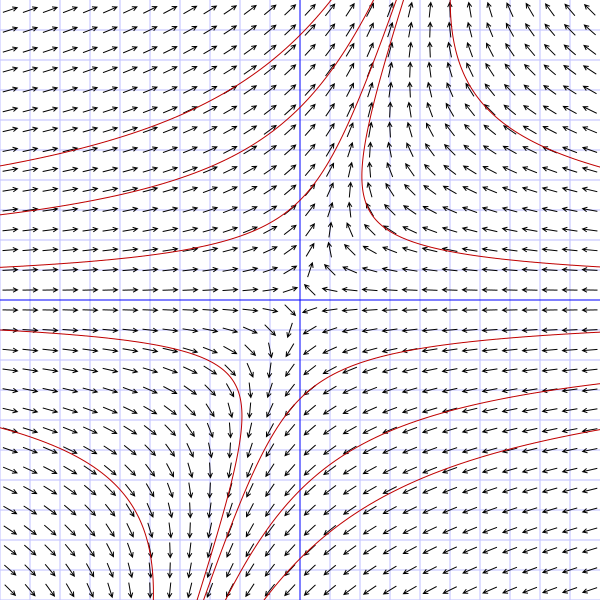
\includegraphics[width=.8\textwidth]{./images/fases-neg-pos.png}
      \caption{$(x', y') = (-2x +y, y)$.}
      \label{fig:fases:neg-pos}
    \end{subfigure}
    \begin{subfigure}{.45\textwidth}
      \centering
      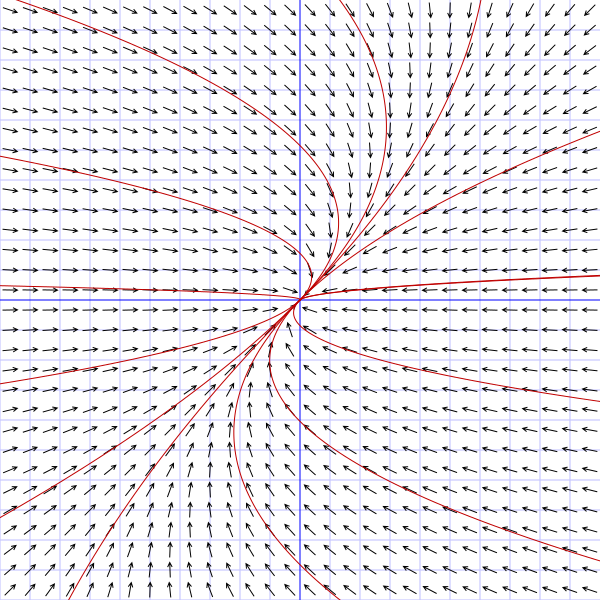
\includegraphics[width=.8\textwidth]{./images/fases-neg-neg.png}
      \caption{$(x', y') = (-2x +y, y)$.}
      \label{fig:fases:neg-neg}
    \end{subfigure}
    \begin{subfigure}{.45\textwidth}
      \centering
      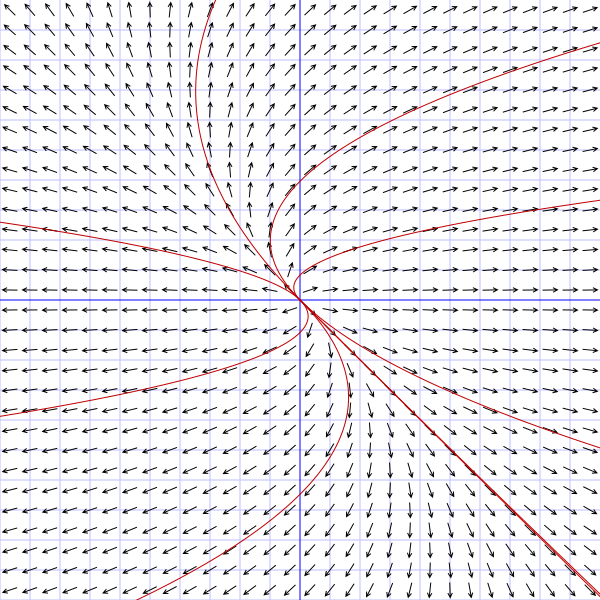
\includegraphics[width=.8\textwidth]{./images/fases-pos-pos.png}
      \caption{$(x', y') = (2x +y, y)$.}
      \label{fig:fases:pos-pos}
    \end{subfigure}
    \begin{subfigure}{.45\textwidth}
      \centering
      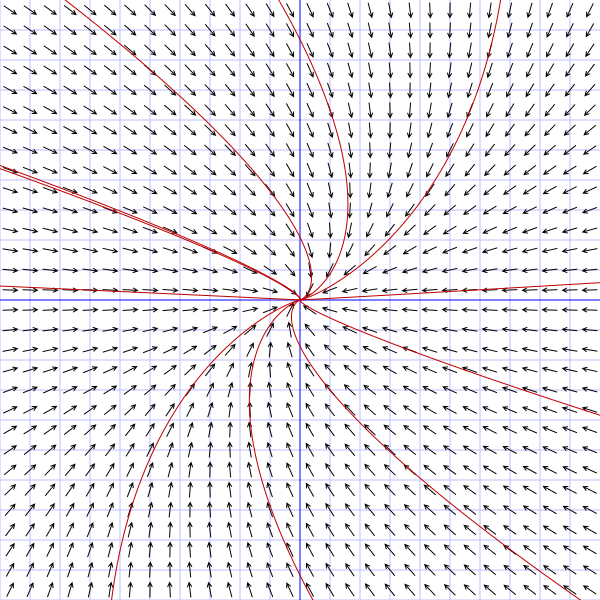
\includegraphics[width=.8\textwidth]{./images/fases-neg-eq.png}
      \caption{$(x', y') = (-2x +y, -2y)$.}
      \label{fig:fases:neg-eq}
    \end{subfigure}
    \caption{Diagramas de fases del sitema \eqref{eq:lineal:cons} cuando los valores propios son
      reales.}
  \end{figure}

\item Los valores propios son complejos. En tal caso, estos son de la forma $\lambda_1 = a+ib$ y
  $\lambda_2 = a-ib$ con $a,b \in \R$. Obtenemos que las soluciones se escriben como
  $\exp(at)( \cos(bt) v_1 + \sin(bt) v_2$. En vista de este hecho, obtenemos los siguientes
  comportamientos.
  \begin{enumerate}[label=\arabic*.]
  \item Si $a = 0$, entonces las componentes de las soluciones son combinaciones lineales de senos y
    cosenos y, por tanto, las soluciones son periódicas y su imagen es una elipse (Figura
    \ref{fig:fases:elip}).
  \item Si $a > 0$, entonces las soluciones tienen a $0$ cuando $t = -\infty$ y divergen cuando
    $t = +\infty$. La imagen de las soluciones forma una espiral en el plano (Figura \ref{fig:fases:espiral:+}).
  \item Si $a z 0$, entonces las soluciones tienen a $0$ cuando $t = +\infty$ y divergen cuando
    $t = -\infty$. La imagen de las soluciones forma una espiral en el plano (Figura \ref{fig:fases:espiral:-}).
  \end{enumerate}
  \begin{figure}[H]
    \centering
    \begin{subfigure}{.45\textwidth}
      \centering
      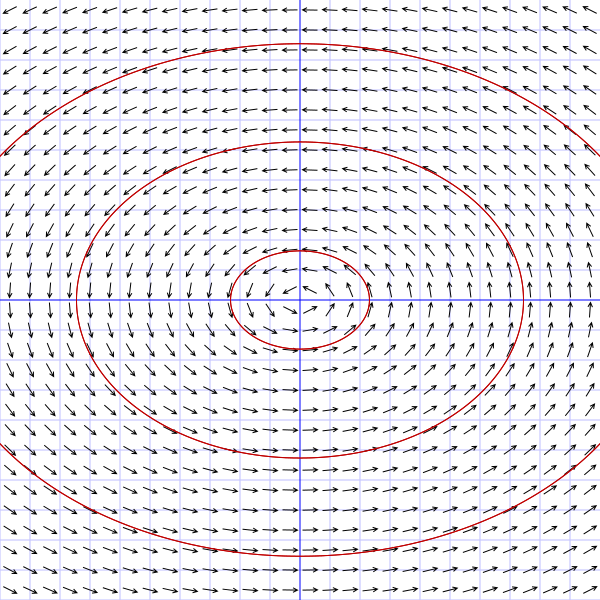
\includegraphics[width=.8\textwidth]{./images/fases-elip.png}
      \caption{$(x', y') = (-2y, x)$.}
      \label{fig:fases:elip}
    \end{subfigure}
    \begin{subfigure}{.45\textwidth}
      \centering
      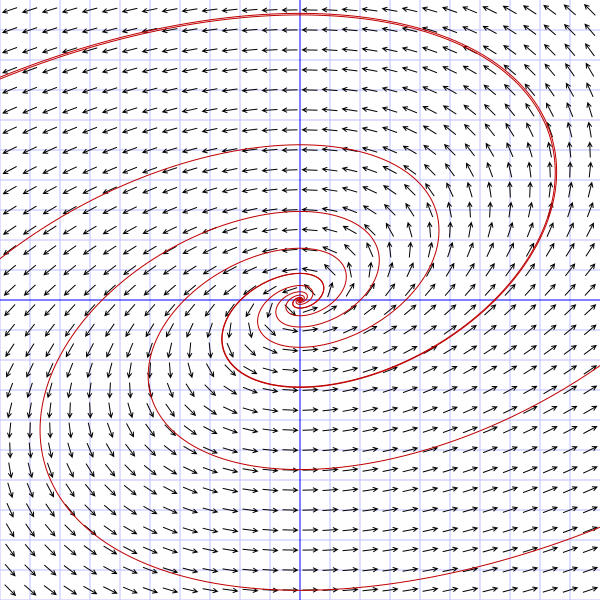
\includegraphics[width=.8\textwidth]{./images/fases-espiral+.png}
      \caption{$(x', y') = (-2y+x, x)$.}
      \label{fig:fases:espiral:+}
    \end{subfigure}
    \begin{subfigure}{.45\textwidth}
      \centering
      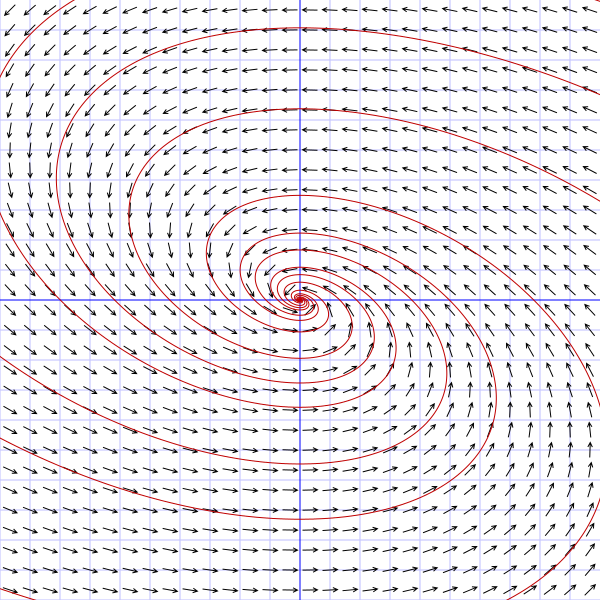
\includegraphics[width=.8\textwidth]{./images/fases-espiral-.png}
      \caption{$(x', y') = (-2y-x, x)$.}
      \label{fig:fases:espiral:-}
    \end{subfigure}
    \caption{Diagramas de fases del sitema \eqref{eq:lineal:cons} cuando los valores propios son
      complejos.}
  \end{figure}
\end{enumerate}


\subsection{El primer método de Lyapunov}

Sea $D \subset \R^d$ abierto y $f \in \mathcal{C}^1(D, \R^d)$. Sea $p \in D$ tal que $f(p) = 0$. La
ecuación \eqref{eq:edo:ae} puede escribirse de la forma
\begin{equation}
  \label{eq:3}
  x' = f'(p)x - f'(p)p + R(x),
\end{equation}
con $||R(x)|| / ||x-p|| \to 0$ cuando $x\to p$.

\begin{theorem}[Primer método de Liapunov]
  \label{thm:lyapunov}
  Sea $D \subset \R^d$ abierto y $f \in \mathcal{C}^1(D, \R^d)$. Consideramos la ecuación
  \eqref{eq:edo:ae}.  Sea $p \in D$ con $f(p) = 0$. Sea
  $\mu = \max \{\mathrm{Re}(\lambda) \mid \lambda \in \sigma(f'(p))\}$.
  \begin{enumerate}
  \item Si $\mu < 0$, entonces $p$ es asintóticamente estable.
  \item Si $\mu > 0$, entonces $p$ es inestable.
  \end{enumerate}
\end{theorem}

\begin{ex}
  
  \begin{enumerate}
  \item Consideramos la EDO $x' = -x^3$. El único punto de equilibrio es $p = 0$, que es un atractor
    global. Nótese que $\mu = 0$ y el sistema es asintóticamente estable.
  \item Consideramos la EDO $x' = x^3$. El único punto de equilibrio es $p = 0$, que es un repulsor
    global. Nótese que $\mu = 0$ y el sistema es inestable.
  \item Consideramos la EDO \eqref{eq:edo:ae} asociada a $f(x) = x^3 \sin(1/x)$. Existe una sucesión
    $\{p_n\}$ de puntos de equilibrios convergentes a $0$. Por tanto, $0$ es estable pero no
    asíntóticamente estable.
  \end{enumerate}
\end{ex}

\begin{corollary}
  Si $d = 2$, en el contexto del Teorema \ref{thm:lyapunov} se verifican las siguientes
  afirmaciones.
  \begin{enumerate}
  \item Si $\det(f'(p)) > 0$ y $\mathrm{traza}(f'(p)) < 0$, entonces $p$ es asintóticamente estable
    para $x' = f(x)$.
  \item Si $\det(f'(p)) < 0$ o $\mathrm{traza}(f'(p)) > 0$, entonces $p$ es inestable.
  \end{enumerate}
\end{corollary}

\begin{ex}[Examen final, 2017]
  Dado el sistema cooperativo
  \begin{equation}
    \label{eq:cooperativo}
    \begin{cases}
      x' = (100 − 20 x + 10 y)x;\\
      y' = (300 + 10 x − 30 y)y.
    \end{cases}
  \end{equation}
  \begin{enumerate}
  \item \textbf{Calcula los puntos de equilibrio.} Tenemos que
    $f(x,y) = ((100-20x+10y)x, (300+10x-30y)y)$. Es fácil ver que los únicos ceros de $f$ son
    $\{(0,0), (0,10), (5,0), (12,14)\}$.
  \item \textbf{Estudia las propiedades de estabilidad de los puntos de equilibrio.} Nótese que la
    matriz jacobiana de $f$ viene dada por
    \[ f'(x,y) = \left( \begin{matrix}
          100 -40x +10y & 10x \\
          10x & 300 +10x-60y
        \end{matrix} \right).

    \]
    \begin{itemize}
    \item En $(0,0)$ tenemos $\mathrm{traza}(f'(0,0)) > 0$, luego es inestable.
    \item En $(0,10)$ se cumple $\det(f'(0,10)) > 0$, luego es inestable.
    \item En $(5,0)$ obtenemos $\det(f'(5,0)) < 0$, luego es inestable.
    \item En $(12,14)$ se tiene $\det(f'(12,14)) > 0$ y $\mathrm{traza}(f'(12,14)) < 0$, por lo que
      el punto de equilibrio es asintóticamente estable. \qedhere
    \end{itemize}
  \end{enumerate}
\end{ex}

En este punto introducimos algunos diagramas de fases en el plano. (Foto de Marta).

\begin{itemize}
\item Heteroclina
\item Homoclina
\item Ciclo límite
\end{itemize}


El problema $16$ de Hilbert se enmarca en este ámbito de las ecuaciones diferenciales. Todavía no
está resuelto. Sean $p,q \in \mathbb{P}_n[x,y]$. Consideramos el sistema
\begin{equation}
  \label{eq:hilbert}
  \begin{cases}
    x' = p(x,y);\\
    y' = q(x,y).
  \end{cases}
\end{equation}
Sea $Z_n$ el número máximo de ciclos límite que puede tener esa familia. El problema 16 de Hilbert
consiste en encontrar una cota superior para $Z_n$.

\begin{ex}[Estabilidad en la ecuación del péndulo]
  Sea $c \ge 0$. Consideramos la ecuación del péndulo
  \begin{equation}
    \label{eq:pendulo:estabilidad}
    x'' + cx' + \sin(x) = 0,
  \end{equation}
  que equivale al sistema
  \begin{equation}
    \label{eq:pendulo:estabilidad:2}
    x_1'' = x_2; \\
    x_2' = - c x_2 - \sin(x_1).
  \end{equation}
  Los puntos de equilibrio del sistema son $\{(k \pi , 0) \mid k \in \Z\}$. Calculamos la matriz
  jacobiana de $f$ , obteniendo
  \[ f'(k\pi, 0) = \left(
      \begin{matrix}
        0 & 1 \\
        \cos(x_1) & -c
      \end{matrix}
    \right). \] Distinguimos dos casos.
  
  \begin{enumerate}
  \item El entero $k$ es par. Deducimos que
    \[ f'(k\pi, 0) = \left(
        \begin{matrix}
          0 & 1 \\
          -1 & -c
        \end{matrix}
      \right) \] y, por tanto, $\det f'(k \pi, 0) = 1 > 0$ y $\mathrm{traza}(f'(k\pi,0)) = -c$. Si
    $c > 0$, entonces el sistema es asintóticamente estable. No obstante, si $c=0$, entonces no
    podemos aplicar el primer método de Lyapunov. Para estos casos existe el segundo método de
    Liapunov, que introduciremos en la siguiente sección.
  \item El entero $k$ es impar. Deducimos que
    \[ f'(k\pi, 0) = \left(
        \begin{matrix}
          0 & 1 \\
          1 & -c
        \end{matrix}
      \right) \] y, por tanto, $\det f'(k \pi, 0) = -1 < 0$ y $\mathrm{traza}(f'(k\pi,0)) = -c$. Por
    tanto, el sistema es inestable. \qedhere
  \end{enumerate}
\end{ex}


\subsection{El segundo método de Lyapunov}

Sea $D \subset \R^d$ un abierto y $f \in \mathcal{C}(D, \R^d)$. Sea $p \in D$ un cero de
$f$. Suponemos que $f$ es localmente lipschitziana Introducimos la siguiente terminología. Sea
$U \subset \R^d$ un entorno de $p \in \R^d$, una función $V \colon U \to \R$ es \emph{definida
  positiva en $U$} si $V(x) > 0$ para todo $x \in U \setminus \{p\}$ y $V(p) = 0$.

\begin{theorem}[Estabilidad de Lyapunov] \label{thm:lyapunov:2} Sea $D \subset \R^d$ un abierto y
  $f \in \mathcal{C}(D, \R^d)$ localmente lipschitziana. Sea $p \in D$ un cero de $f$. Si existe una
  función $V \in \mathcal{C}^1(D)$ tal que $V$ alcanza un mínimo local estricto en $p$ y existe un
  entorno $U \subset D$ de $p$ tal que $\dot{V}(x) \le 0$ para todo $x \in U$. Entonces, $p$ es un
  punto de equilibrio estable de \eqref{eq:edo:ae}.
\end{theorem}
\begin{proof}
  Por hipótesis existe $0 < R$ tal que $V(x) > V(p)$ y $\dot{V}(x) \le 0$ para todo
  $x \in \overline{\mathrm{B}}(p, R) \setminus \{p\}$. Sea $\varepsilon > 0$. No es restrictivo
  suponer que $\varepsilon \le R$. Sea
  $m = \min \{V(x) \mid x \in \partial \mathrm{B}(p,\varepsilon)\}$. Por continuidad de $V$ existe
  $\delta > 0$ tal que para todo $x \in \mathrm{B}(p, \delta)$ se cumple $V(x) < m$. Sea
  $x_0 \in \mathrm{B}(p, \delta)$. Vamos aprobar que la solución $X(t,0,x_0) = X(t,x_0)$ verfica
  $X(t, x_0) \in \mathrm{B}(p,\varepsilon)$ para todo $t \ge 0$. Razonamos por reducción al
  absurdo. Existe $\tau > 0$ tal que $X(t, x_0) \in \mathrm{B}(p,\varepsilon)$ para todo
  $t \in [0, \tau[$ y $X(\tau, x_0) \in \partial \mathrm{B}(p,\varepsilon)$. La función
  $y(t) = V(X(t,x_0))$ es decreciente pues $y'(t) = \dot{V}(X(t,x_0)) \le 0$. Sin embargo,
  $y(\tau) \ge m > V(x_0) = y(0)$, contradicción. Por tanto, por el teorema de comportamiento en el
  extremo superior $\omega(0, x_0) = +\infty$ y $||X(t, x_0) - p|| \le \varepsilon$ para todo
  $t \in [0,+\infty[$, $x_0 \in \mathrm{B}(p,\delta)$.
\end{proof}

\begin{corollary}
  Sea $D \subset \R^d$ un abierto y $f \in \mathcal{C}(D, \R^d)$ localmente lipschitziana. Sea
  $p \in D$ un cero de $f$. Si existe una función $V \in \mathcal{C}^1(D)$ tal que $V$ alcanza un
  mínimo local estricto en $p$ y existe un entorno $U \subset D$ de $p$ tal que $\dot{V}(x) = 0$
  para todo $x \in U$. Entonces, $p$ es un punto de equilibrio estable pero no asintóticamente
  estable de \eqref{eq:edo:ae}.
\end{corollary}
\begin{proof}
  Supongamos que para cierto $x_0 \in D$ se tiene que $\lim_{t \to \omega} X(t,x_0) = p$. En tal
  caso, la función $y(t) = V(X(t,x_0))$ tiene derivada constantemente cero para $t$ lo
  suficientemente grande. Sin embargo, $X(t,x_0) \ne p$ para todo $t\in ]\alpha,\omega[$, lo que
  contradice que $V$ tenga un mínimo local estricto en $p$.
\end{proof}

\begin{ex}[Estabilidad en la ecuación del péndulo, 2]
  Recuperamos la ecuación del péndulo \eqref{eq:pendulo:estabilidad} y su versión en sistema
  \eqref{eq:pendulo:estabilidad:2}. Recordemos que los puntos de equilibio son
  $\{(k \pi, 0) \mid k \in \Z\}$. Habíamos estudiado la estabilidad en todos los casos salvo cuando
  $k$ es par y $c = 0$. En tal caso, la ecuación a estudiar es la siguiente
  \begin{equation}
    \label{eq:pendulo:estabilidad:3}
    \begin{cases}
      x_1' = x_2; \\
      x_2' = - \sin(x_1).
    \end{cases}
  \end{equation}
  Definimos $V \colon \R^2 \to \R$ dada por $V(x,y) = y^2 /2 - \cos(x)$. Tenemos que
  $\dot{V}(x,y) = 0$. Además, $V$ alcanza un mínimo local estricto en $(0,0)$. Por tanto, el segundo
  método de Lyapunov nos asegura que \eqref{eq:pendulo:estabilidad:3} es estable.
\end{ex}

El problema del Teorema de Estabilidad de Lyapunov es encontrar una función $V$ apropiada. En el
caso de los sistemas del tipo lineal \eqref{eq:....} $x' = A x$. En tal caso podremos encontrar una
forma cuadrática que verifique estas condiciones. Sea $B \in \mathcal{M}_d(\R)$ simétrica. La forma
cuadrática asociada es $V(x) = \left\langle Bx, x \right\rangle$. La función $V$ tiene un mínimo
estricto en $0$ si, y solo si, es definida positiva. Recordemos que $\nabla V(x) = 2 Bx$. Por tanto,
tenemos que
\[\dot{V}(x) = \left\langle 2 B x, Ax \right\rangle = 2 \left\langle A^{t} Bx, x \right\rangle =
  \left\langle \frac{A^{t}B + B A}{2} x, x\right\rangle.\] Por tanto, el hecho de que
$\dot{V}(x) \le 0$ para todo $x$ equivale a que la matriz $A^{t}B + B A$ (parte simétrica de $BA$)
sea semidefinida negativa. Definimos $F_A \colon \mathrm{S}^+_d \to \mathrm{S}_d(\R)$ dada por
$F_A(B) = A^{t}B+BA$. Esta aplicación es lineal. Consecuentemente, interesa conocer las propiedades
de $F_A$ de manera que dada una matriz definida negativa podamos calcular su imagen inversa por
$F_A$.

Es fácil demostrar el siguiente lema.
\begin{lemma}
  Sea $\varphi \colon ]\alpha, +\infty[ \to \R^d$ continua. Supongamos que se verifican las
  siguientes hipótesis.
  \begin{enumerate}
  \item Existe $R > 0$ y $t_0 > \alpha$ tal que $\varphi(t) \in \overline{\mathrm{B}}(p,R)$ para
    todo $t \ge t_0$.
  \item Existe $V \in \mathcal{C}(\overline{\mathrm{B}}(p,R))$ tal que $V(x) > V(p)$ para todo
    $x \in \overline{\mathrm{B}}(p,R)\setminus \{p\}$.
  \item $\lim_{t \to +\infty} V(\varphi(t)) = V(p)$.
  \end{enumerate}
  Entonces $\lim_{t \to +\infty} \varphi(t) = p$.
\end{lemma}

Como consecuencia podemos demostrar el segundo resultado de estabilidad asintoica de Liapunov
\begin{theorem}[Estabilidad asintótica de Liapunov - 2]
  \label{thm:lyapunov:3}
  Sea $D \subset \R^d$ un abierto y $f \in \mathcal{C}(D, \R^d)$ localmente lipschitziana. Sea
  $p \in D$ un cero de $f$.  Sea $V \in \mathcal{C}^1(D)$ tal que $V$ alcanza en $p \in D$ un mínimo
  local estricto. Si $\dot{V}$ alcanza un máximo local estricto en $p$, entonces $p$ es un punto de
  equilibrio asintóticamente estable de \eqref{eq:edo:ae}.
\end{theorem}
\begin{proof}
  Por el Teorema \ref{thm:lyapunov:2} tenemos que $p$ es un punto de equilibrio estable de
  \eqref{eq:edo:ae}. Sea $R > 0$ tal que $V$ tiene un mínimo global y $\dot{V}$ tiene un máximo
  global en $\mathrm{B}(p, R)$. Por la estabilidad existe un $\mu > 0$ tal que para todo
  $x_0 \in \mathrm{B}(p,\mu)$ se tiene $\omega(x_0) = +\infty$ y $X(t, x_0) \in \mathrm{B}(p, R)$
  para todo $t \ge 0$. Sea $\varphi(t) = X(t, x_0)$ e $y(t) = V(\varphi(t))$. Nótese que
  $y'(t) = \dot{V}(\varphi(t)) \le 0$ para todo $t \ge 0$. Por tanto, $y$ es decreciente y está
  acotada inferiormente por $V(p)$. Deducimos que existe $L = \lim_{t \to +\infty} y(t) \ge
  V(p)$. Veamos que $L = V(p)$. Por el teorema del valor medio obtenemos una sucesión de números no
  negativos $\{t_n\}\to+\infty$ tal que $\{\dot{V}(\varphi(t_n))\} = \{y'(t_n)\}\to 0$. Pero
  $\dot{V}$ tiene un máximo estricto en $p$ y $\varphi(t_n) \in \mathrm{B}(p, R)$, luego
  $\{\varphi(t_n)\} \to p$ y, por tanto, $\{V(\varphi(t_n))\} \to V(p)$. La unicidad del límite
  prueba que $L = V(p)$. La demostración finaliza al aplicar el lema previo.
\end{proof}

El teorema previo se suele aplicar utilizando las conocidas condiciones suficientes de mínimo y
máximos estrictos en funciones de clase 1. No obstante, las hipótesis son muy restrictivas y no
cubren todos los casos, como muestra el siguiente ejemplo.

\begin{ex}
  Consideramos la EDO $x'' + x' + x^3 = 0$. Esta se denomina ecuación de Duffing. El sistema
  asociado viene dado por
  \[
    \begin{cases}
      x_1' = x_2;\\
      x_2' = - x_1^3 - x_2.
    \end{cases}
  \]
  El único punto de equilibrio es el $(0,0)$. Nótese que $\mathrm{traza}(f'(0,0)) < 0$ y
  $\det(f'(0,0)) = 0$, por lo que el primer método de Liapunov no da información acerca de la
  estabilidad en $(0,0)$. Buscamos pues aplicar el segundo método. Consideramos la función energía
  $V(x_1, x_2) = x_1^4 / 4 + x_2^2 / 2$, que tiene un mínimo global estricto en $(0,0)$. Tenemos que
  $\dot{V}(x_1, x_2) = -x_2^2$, que tiene un máximo en $(0,0)$, pero no es estricto en ningún
  entorno. Deducimos que el punto de equilibrio es estable por el Teorema \ref{thm:lyapunov:2}, pero
  no sabemos si es asintóticamente estable o no. No obstante, sí se puede demostrar que el
  equilibrio es asintóticamente estable. En efecto, basta considerar una nueva función
  $V(x_1, x_2) = x_1^4 / 4 + x_2^2 / 2 + ax_1^3 x_2$. Se deja como ejercicio encontrar un valor de
  $a$ para el cual se pueda aplicar el Teorema \ref{thm:lyapunov:3}.
\end{ex}

\begin{theorem} [Inestabilidad de Lyapunov]
  \label{thm:lyapunov:5}
  Sea $D \subset \R^d$ un abierto y $f \in \mathcal{C}(D, \R^d)$ localmente lipschitziana. Sea
  $p \in D$ un cero de $f$.  Sea $V \in \mathcal{C}^1(D)$ tal que existe una sucesión
  $\{s_n\} \subset D$ convergente a $p$ tal que $V(x_n) > 0$ para todo $n \in \N$. Si $\dot{V}$
  alcanza un mínimo local estricto en $p$, entonces $p$ es un punto de equilibrio inestable de
  \eqref{eq:edo:ae}.
\end{theorem}
\begin{proof}
  Sea $R > 0$ tal que $V$ y $\dot{V}$ tienen un máximo global estricto en $p$ en
  $\mathrm{B}(p,R)$. Supongamos que $p$ es estable y lleguemos a una contradicción. En tal caso
  existe $\mu > 0$ tal que para todo $x_0 \in \mathrm{B}(p,\mu)$ se tiene que
  $\omega(x_0) = +\infty$ y $X(t;x_0) \in \overline{\mathrm{B}(p,R)}$ para todo $t \ge 0$. Sea
  $x_0 \in \mathrm{B}(p,R) \setminus \{p\}$ y $\varphi(t) = X(t, x_0)$. Se tiene que
  $\varphi(t) \ne p$ para todo $t \in ]\alpha(x_0),+\infty[$.  Definimos la función
  $y(t) = V(\varphi(t))$. Tenemos que $y'(t) = \dot{V}(\varphi(t)) > 0$ para todo $t \ge 0$, luego
  la función $y$ es estrictamente creciente. Consecuentemente, existe
  $L = \lim_{t \to +\infty} V(\varphi(t)) > V(x_0)$, de donde encontramos una sucesión de números no
  negativos $\{t_n\}$ tal que $\{\dot{V}(\varphi(t_n))\} = \{y'(t_n)\} \to 0$. Por continuidad de
  $V$, existe $\delta >0$ tal que $V(x) < r$ para todo $\mathrm{B}(p,\delta)$. Deducimos que
  $\varphi(t) \in \overline{\mathrm{B}}(p, R) \setminus \mathrm{B}(p, \delta)$. No obstante, tenemos
  que $m = \min \{\dot{V}(x) : x \in \overline{\mathrm{B}}(p,R) \setminus \mathrm{B}(p,\delta)\}$ >
  0, luego existe $N \in \N$ tal que $y'(t_N) < m$. Deducimos que
  $\varphi(t_N) \in \mathrm{B}(p,\delta)$, contradicción.
\end{proof}

\begin{corollary}
  Sea $D \subset \R^d$ un abierto y $f \in \mathcal{C}(D, \R^d)$ localmente lipschitziana. Sea
  $p \in D$ un cero de $f$.  Sea $V \in \mathcal{C}^1(D)$ tal que $V$ alcanza en $p \in D$ un mínimo
  local estricto. Si $\dot{V}$ alcanza un mínimo local estricto en $p$, entonces $p$ es un punto de
  equilibrio inestable de \eqref{eq:edo:ae}. Es más, si $D = \R^d$, entonces ninguna solución está
  acotada.
\end{corollary}

Un teorema complementario al Teorema \ref{thm:lyapunov:5} es el siguiente resultado.

\begin{theorem} [Inestabilidad de Chetaev]
  \label{thm:chetaev}
  Sea $D \subset \R^d$ un abierto y $f \in \mathcal{C}(D, \R^d)$ localmente lipschitziana. Sea
  $p \in D$ un cero de $f$.  Sea $V \in \mathcal{C}^1(D)$ tal que existe una sucesión
  $\{s_n\} \subset D$ convergente a $p$ tal que $V(x_n) > 0$ para todo $n \in \N$. Si
  $\dot{V}(x) > 0$ para todo $x \in \mathcal{U}_+ = \{x \in D : V(x) > 0\}$.  alcanza un mínimo
  local estricto en $p$, entonces $p$ es un punto de equilibrio inestable de \eqref{eq:edo:ae}.
\end{theorem}

Las funciones $V$ de estos teoremas reciben el nombre de funciones de Lyapunov.

\begin{ex}
  Consideramos el sistema
  
  \begin{equation}
    \label{eq:lyapunov}
    \begin{cases}
      x' = y - x(1+|y|);\\
      y ' = x + y (1+|y|).
    \end{cases}
  \end{equation}
  Estudiar la estabilidad de \eqref{eq:lyapunov} en los puntos de equilibrio.

  El único punto de equilibrio es $p = (0,0)$. La función $V(x,y) = xy$ verifica las hipótesis del
  Teorema \ref{thm:lyapunov:5}, luego $p$ es inestable.
\end{ex}

\subsection{Sistemas gradientes}


\subsubsection{Sistemas gradientes de primer orden}

Sea $D \subset \R^d$ un abierto y $G \in \mathcal{C}^1(D)$. Sea $p \in D$ tal que $\nabla G(p) =
0$. Consideramos el sistema
\begin{equation}
  \label{eq:gradiente:1}
  x´ + \nabla G (x) = 0.
  \tag{G1}
\end{equation}

\begin{proposition} \label{prop:gradiente:1} En el contexto actual suponemos que $p$ es un punto
  crítico aislado de $f(x) = - \nabla G(x)$.
  \begin{enumerate}
  \item Si $G$ alcanza en $p$ un mínimo local estricto, entonces $p$ es un punto de equilibrio
    asintóticamente estable de \eqref{eq:gradiente:1}.
  \item Si $G$ alcanza en $p$ un máximo local estricto, entonces $p$ es un punto de equilibrio
    inestable de \eqref{eq:gradiente:1}.
  \item Si $G$ alcanza en $p$ un punto de silla, entonces $p$ es un punto de equilibrio inestable de
    \eqref{eq:gradiente:1}.
  \end{enumerate}
\end{proposition}
\begin{proof}
  La idea es aplicar los resultados de Lyapunov para funciones basadas en $G$.
  
  \begin{enumerate}
  \item Basta considerar $V(x) = G(x)$ y aplicar el Teorema \ref{thm:lyapunov:2} pues
    $\dot{V}(x) = \left\langle \nabla G(x), -\nabla G(x) \right\rangle = - ||\nabla G(x)||^2$.
  \item Consideramos en este caso $V(x) = - G(x)$ y aplicamos el Teorema \ref{thm:lyapunov:3}.
  \item Consideramos de nuevo $V(x) = - G(x)$ y aplicamos el Teorema \ref{thm:chetaev}. \qedhere
  \end{enumerate}
\end{proof}

La dificultad de utilizar este resultado reside en saber si el sistema con el que estamos trabajando
es un sistema gradiente. Para ello utilizamos el lema de Schwarz como muestra el siguiente ejemplo.

\begin{ex}
  Consideramos el sitema
  
  \begin{equation}
    \label{eq:schwarz}
    \begin{cases}
      x' = 28x - 6x^2 + 4y; \\
      y' = 4y +4x.
    \end{cases}
  \end{equation}
  ¿Es un sistema gradiente? Sea $f_1(x,y) = 28x - 6x^2 + 4y$ y $f_2(x,y) = 4y +4x$. En caso de ser
  un sistema gradiente se tendrá $\frac{\partial}{\partial y} f_1 = \frac{\partial}{\partial x} f_2$
  por el lema de Schwarz. Es fácil comprobar que sto se verifica en el sitema. Ahora podemos
  proceder como sigue. Tomamos $-G(x,y) = 14x^2 - 2x^3 + 4xy + \varphi(y)$, primitiva de $f_1$
  fijando $y$. Calculamos ahora $\varphi(y)$. Para ello derivamos respecto de $y$ obteniendo que
  $4x + \varphi'(y) = 4x+4y = f_2(x,y)$. Deducimos que $\varphi(y) = 2y^2 + k$. Nótese que las $x$
  se han cancelado al calcular $\varphi'$ gracias a que se verifica la tesis del lema de
  Schwarz. Podemos tomar $G(x,y) = - (14x^2-2x³)+4xy+2y^2$.
\end{ex}

\subsubsection{Sistemas gradientes de segundo orden}

Sea $D \subset \R^d$ un abierto y $G \in \mathcal{C}^1(D)$. Sea $p \in D$ tal que $\nabla G(p) =
0$. Un sistema gradiente de segundo orden es una EDO de la forma
\begin{equation}
  \label{eq:gradiente:2}
  x'' + \nabla G(x) = 0.
  \tag{G2}
\end{equation}
Equivalentemente, podemos considerar el sistema
\begin{equation}
  \label{eq:gradiente:2:s}
  \begin{cases}
    x_1' = x_2; \\
    x_2' = - \nabla G(x_1).
  \end{cases}
  \tag{G2S}
\end{equation}

\begin{theorem}
  \label{thm:lagrange-dirichlet}
  En el contexto actual, si $G$ alcanza en $p$ un mínimo local estricto, entonces $(p,0)$ es un
  punto de equilibrio estable pero no asintóticamente estable de \eqref{eq:gradiente:2:s}.
\end{theorem}
\begin{proof}
  Consideramos la función $V(x_1, x_2) = G(x_1) + ||x_2||_2^2 / 2$. Es fácil ver que es una función
  de Lyapunov para el corolario del Teorema \ref{lyapunov:2}. En efecto, se tiene
  $\dot{V}(x_1, x_2) = \left\langle \nabla G(x_1) + x_1+ + x_2, \right\rangle$ terminar....
\end{proof}


%%% Local Variables: ***
%%% mode:latex ***
%%% TeX-master: "../df2.tex"  ***
%%% End: ***
